\subsection*{\textcolor{subsectioncolor}{\textsf{2. \textit{EXTERNAL INTERFACE}}}}
\addcontentsline{toc}{subsection}{2. \textit{EXTERNAL INTERFACE}}


Tampilan antarmuka pengguna terdapat pada subsistem \textit{client},
dan dapat dibagi menjadi tiga, yaitu:
\begin{itemize}
	\item Tampilan jendela saat melakukan \textit{loading} seperti ditunjukan oleh Gambar ~\ref{fig:loading}
	\item Tampilan jendela utama dengam mode jendela (\textit{windowed}) seperti ditunjukan oleh Gambar ~\ref{fig:windowed}
	\item Tampilan jendela utama dengan mode penuh (\textit{fullscreen}) seperti ditunjukan oleh Gambar ~\ref{fig:fullscreen}
\end{itemize}
\begin{figure}
	\centering
		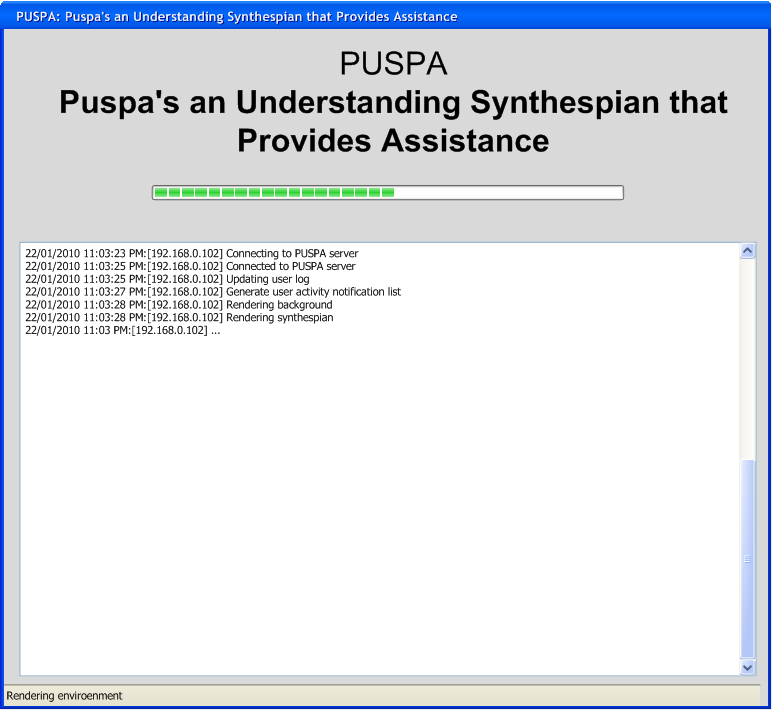
\includegraphics[width=0.6\textwidth]{loading.png}
	\caption{Tampilan antarmuka saat \textit{loading}}
	\label{fig:loading}
\end{figure}
\begin{figure}
	\centering
		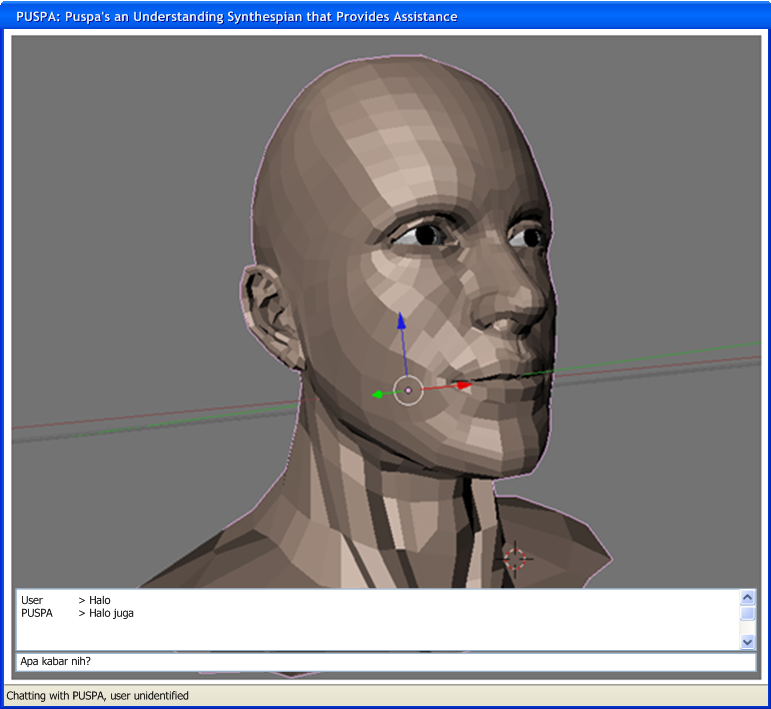
\includegraphics[width=0.6\textwidth]{windowed.png}
	\caption{Tampilan antarmuka dalam jendela (\textit{windowed})}
	\label{fig:windowed}
\end{figure}
\begin{figure}
	\centering
		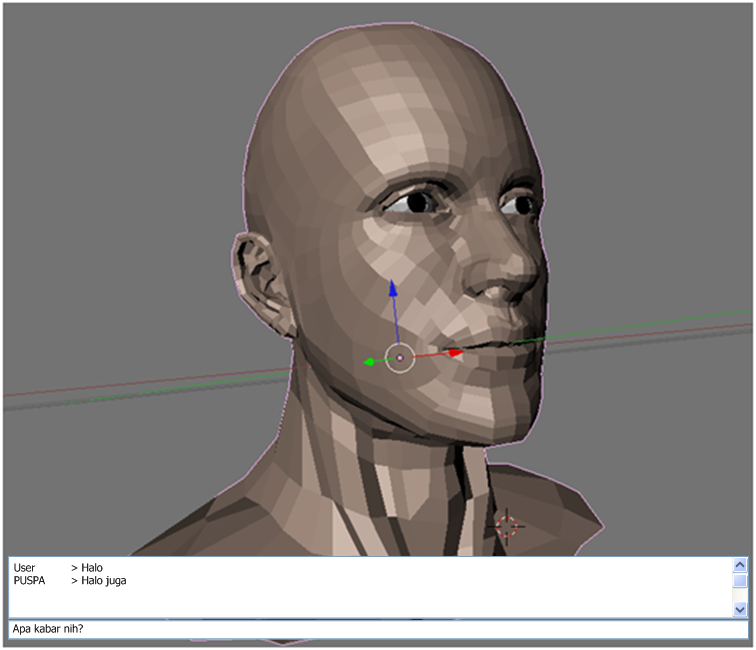
\includegraphics[width=0.8\textwidth]{fullscreen.png}
	\caption{Tampilan antarmuka penuh (\textit{fullscreen})}
	\label{fig:fullscreen}
\end{figure}
